% Header
%%%%%%%%%%%%%%%%%%%%%%%%%%%%%%%%%%%%%%%%%%%%%%%%%%%%%%%%%%%%%%%%%%%%%%%%%%%%%%%%%%%

\chapter{Fundamentals}
\label{fundamentals}
\thispagestyle{empty}

%%%%%%%%%%%%%%%%%%%%%%%%%%%%%%%%%%%%%%%%%%%%%%%%%%%%%%%%%%%%%%%%%%%%%%%%%%%%%%%%%%%


This chapter includes the most important fundamentals about the cardiac anatomy and physiology, as well as the necessary technical background for understanding the methods developed during the research for this master thesis. The first section covers the human physiology.





% First Section: Physiological Fundamentals
%%%%%%%%%%%%%%%%%%%%%%%%%%%%%%%%%%%%%%%%%%%%%%%%%%%%%%%%%%%%%%%%%%%%%%%%%%%%%%%%%%

\section{Physiological Fundamentals}
\label{physiologicalFundamentals}
Looking at a human heart from an engineer's perspective, it can be described as a highly optimized technical systems. The heart is a strong pump with pipes and valves and it is driven by electric excitation. Just like an artificial system it depends on a control unit, which is able to adapt to different conditions and disturbances. Although the human heart is a very robust and durable system, its efficiency and functionality declines with time. On top the components of this complex system might also fail, if they are exposed to too much stress, again just like in an engineered system. 
In order to detect and possibly solve these failures, the Electrocardiogram (ECG) represents a powerful tool. It is measured using electrodes, which record the electrical excitation on the skin.
\newline
This section describes the most important components of this complex object. It is not intended to give a detailed discourse of the anatomy and physiology, yet the section introduces the necessary facts to understand the analysis methods, developed during the research for this thesis. The topics, which will be introduced, include the heart itself and the Autonomic Nervous System (ANS). The respiratory system and its influence on the functionality of the heart is furthermore described. Subsequently an explanation of the Electrocardiogram (ECG) and its interpretation can be found in the last part of this section.

% Anatomy of the Human Heart
% -----------------------------------------------------------------------------------------------------------------------------------------------------------------------------------------------------------------------
\subsection{The Anatomy and Mechanics of the Human Heart}
\label{anatomy}
\textcolor{green}{
	Here I want to have multiple paragraphs:
	\begin{enumerate}
  		\item location of the heart  
  		\item anatomy of the heart
  		\item blood flow (pulmonary circle,systematic circle,Filling-/Emptying phase)
	\end{enumerate}
}
The human heart is a hollow muscle, which establishes the blood supply to all organs in the body. It is the driving force for the blood circulation in the human body and is located in the thoracic cavity, between the breastbone anteriorly and the backbone posteriorly \cite{sherwood07}. The heart has a broad base on the top directly behind the backbone in the middle of the chest, while the tip of the heart, the apex, is pointed away from the middle to the left. The apex can actually bang against the chest, when the heart beats strongly, which explains the misleading feeling of many, that the heart is located in the left half of the thorax \cite{sherwood07}. The organ resembles a human clenched fist in shape and size and weighs about 250 - 400\,g \cite{schwegler11}, depending on the gender, age and physical fitness of the person. \textcolor{red}{Include a picture to show location of the heart and the reference to the picture here.} 
\newline
The heart consists of two halves, left and right. These two individual halves serve as separate pumps, which are again subdivided into a small chamber, the atrium, and a large chamber, the ventricle. A muscular partition separates the two halves, which is formed by the interatrial septum between the left and right atrium and the interventricular septum between the ventricles.
\begin{figure}
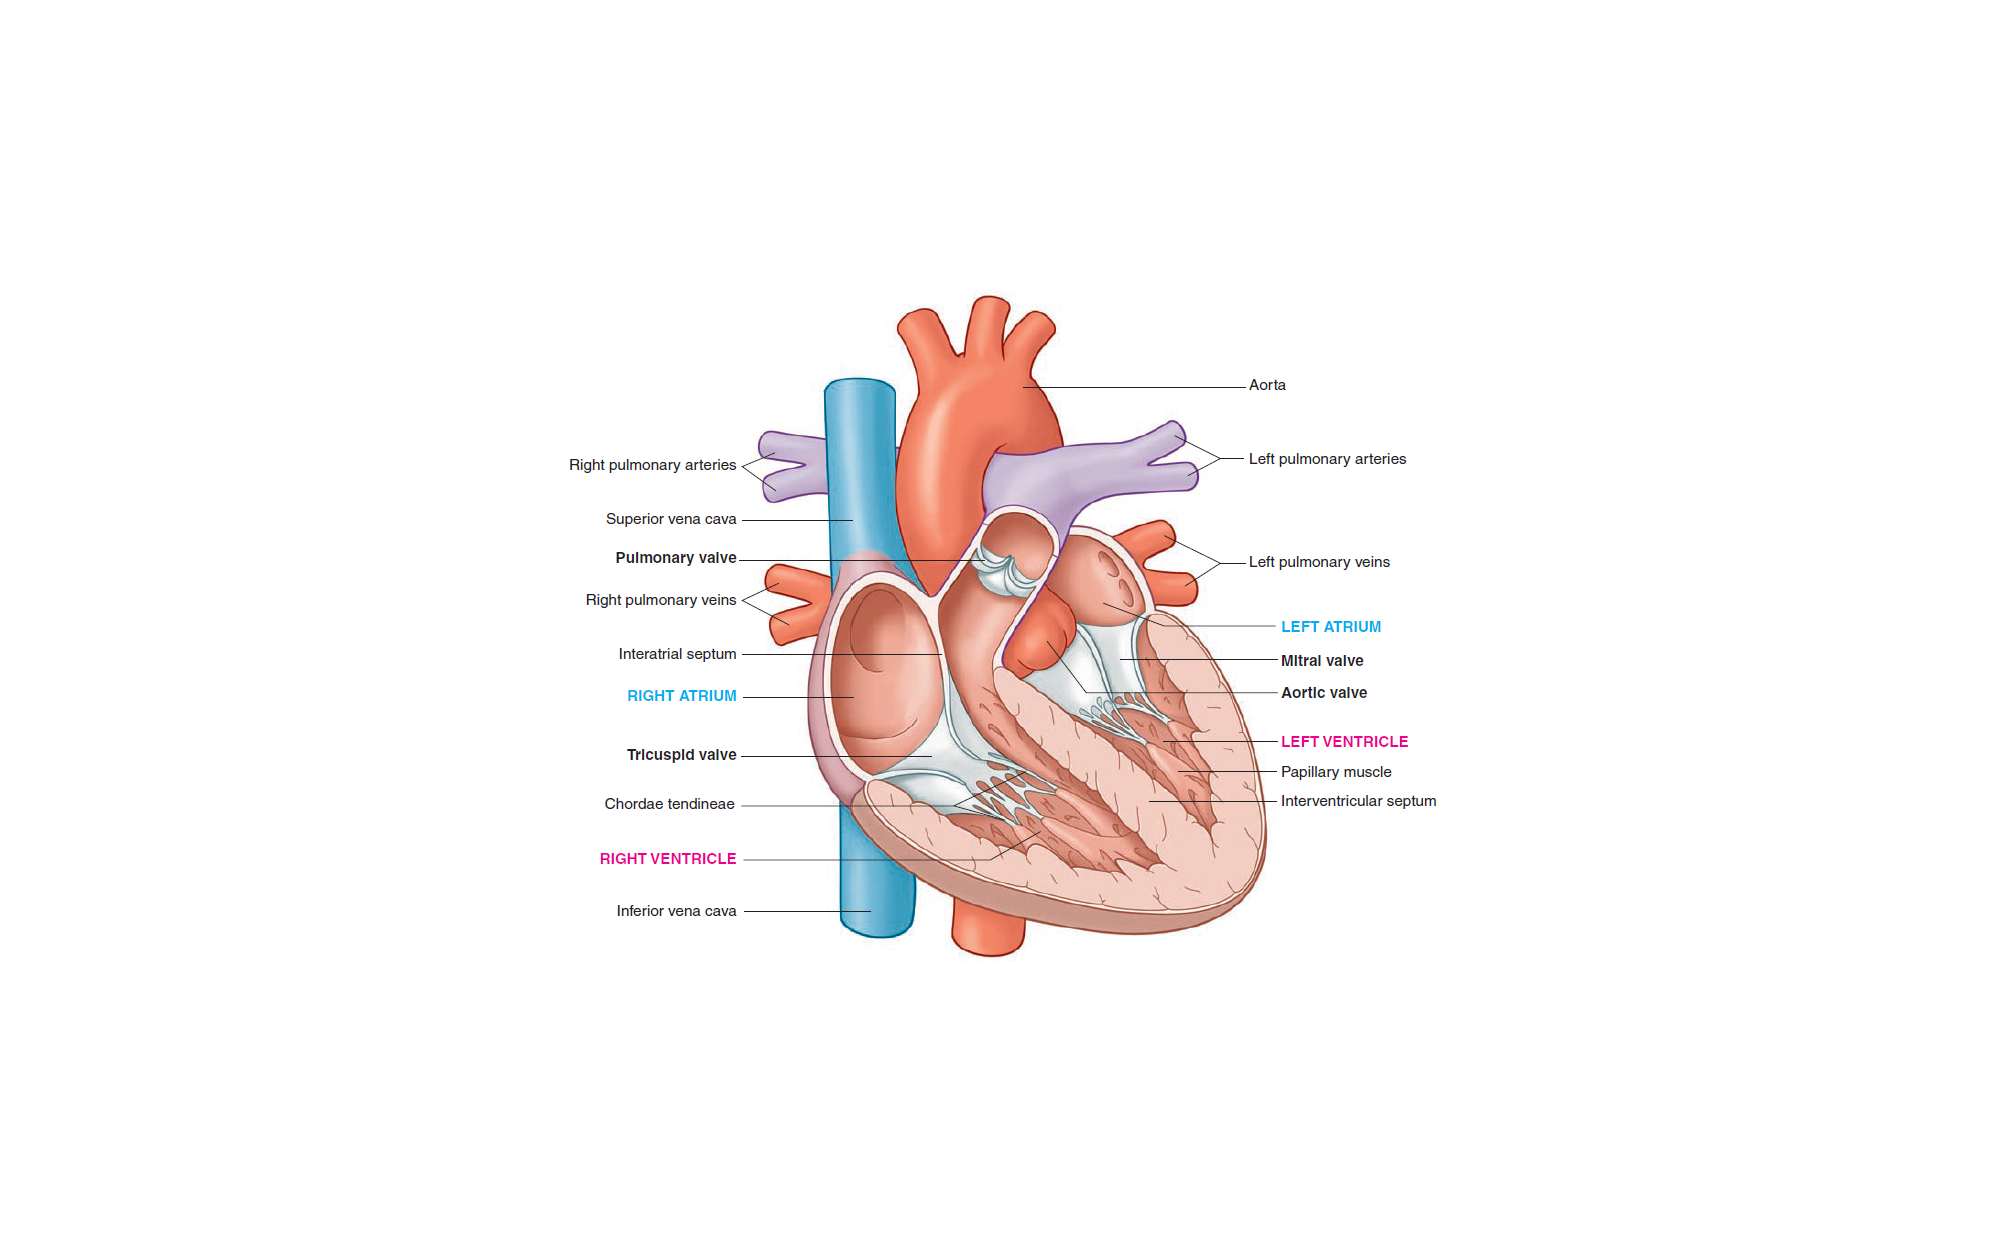
\includegraphics{HeartAnatomy.png}
\end{figure}
\textcolor{red}{Include a picture to show anatomy of the heart and the reference to the picture here.} 
\newline

% -----------------------------------------------------------------------------------------------------------------------------------------------------------------------------------------------------------------------



% Electrophysiology of the Human Heart
% -----------------------------------------------------------------------------------------------------------------------------------------------------------------------------------------------------------------------
\subsection{The Electrophysiology of the Human Heart}
\label{physiology}
% -----------------------------------------------------------------------------------------------------------------------------------------------------------------------------------------------------------------------



% The Autonomic Nervous System
% -----------------------------------------------------------------------------------------------------------------------------------------------------------------------------------------------------------------------
\subsection{The Autonomic Nervous System}
\label{ans}
% -----------------------------------------------------------------------------------------------------------------------------------------------------------------------------------------------------------------------



% The ECG
% -----------------------------------------------------------------------------------------------------------------------------------------------------------------------------------------------------------------------
\subsection{The Electrocardiogram (ECG)}
\label{ecg}
\paragraph{The Vectorcardiogram (VCG)}
\label{vcg}
\paragraph{The Respiratory Sinus Arrhythmia (RSA)}
\label{rsa}
% -----------------------------------------------------------------------------------------------------------------------------------------------------------------------------------------------------------------------

%%%%%%%%%%%%%%%%%%%%%%%%%%%%%%%%%%%%%%%%%%%%%%%%%%%%%%%%%%%%%%%%%%%%%%%%%%%%%%%%%%%





% Second Section: Mathematical Fundamentals
%%%%%%%%%%%%%%%%%%%%%%%%%%%%%%%%%%%%%%%%%%%%%%%%%%%%%%%%%%%%%%%%%%%%%%%%%%%%%%%%%%%

\section{Mathematical Fundamentals}
\label{mathematicalFundamentals}



% Time Continuous and Time Discrete Signals
% -----------------------------------------------------------------------------------------------------------------------------------------------------------------------------------------------------------------------
\subsection{Time Continuous  and Discrete Signals}
\label{contSignal}
% -----------------------------------------------------------------------------------------------------------------------------------------------------------------------------------------------------------------------
\textcolor{green}{
	Here I want to have multiple paragraphs:
	\begin{enumerate}
  		\item cont. and discrete signal basics  
  		\item Energy signals
  		\item Power signals
	\end{enumerate}
}
%%%%%%%%%%%%%%%%%%%%%%%%%%%%%%%%%%%%%%%%%%%%%%%%%%%%%%%%%%%%%%%%%%%%%%%%%%%%%%%%%%%


